\section{Result Graphs}

\subsection{Purpose}

This section presents graphical summaries of the major experimental results. The graphs make it easier to compare convergence time, packet loss, and additional validation evidence across the different routing mechanisms.

\subsection{Convergence and Reaction Time Comparison}

\begin{figure}[H]
\centering
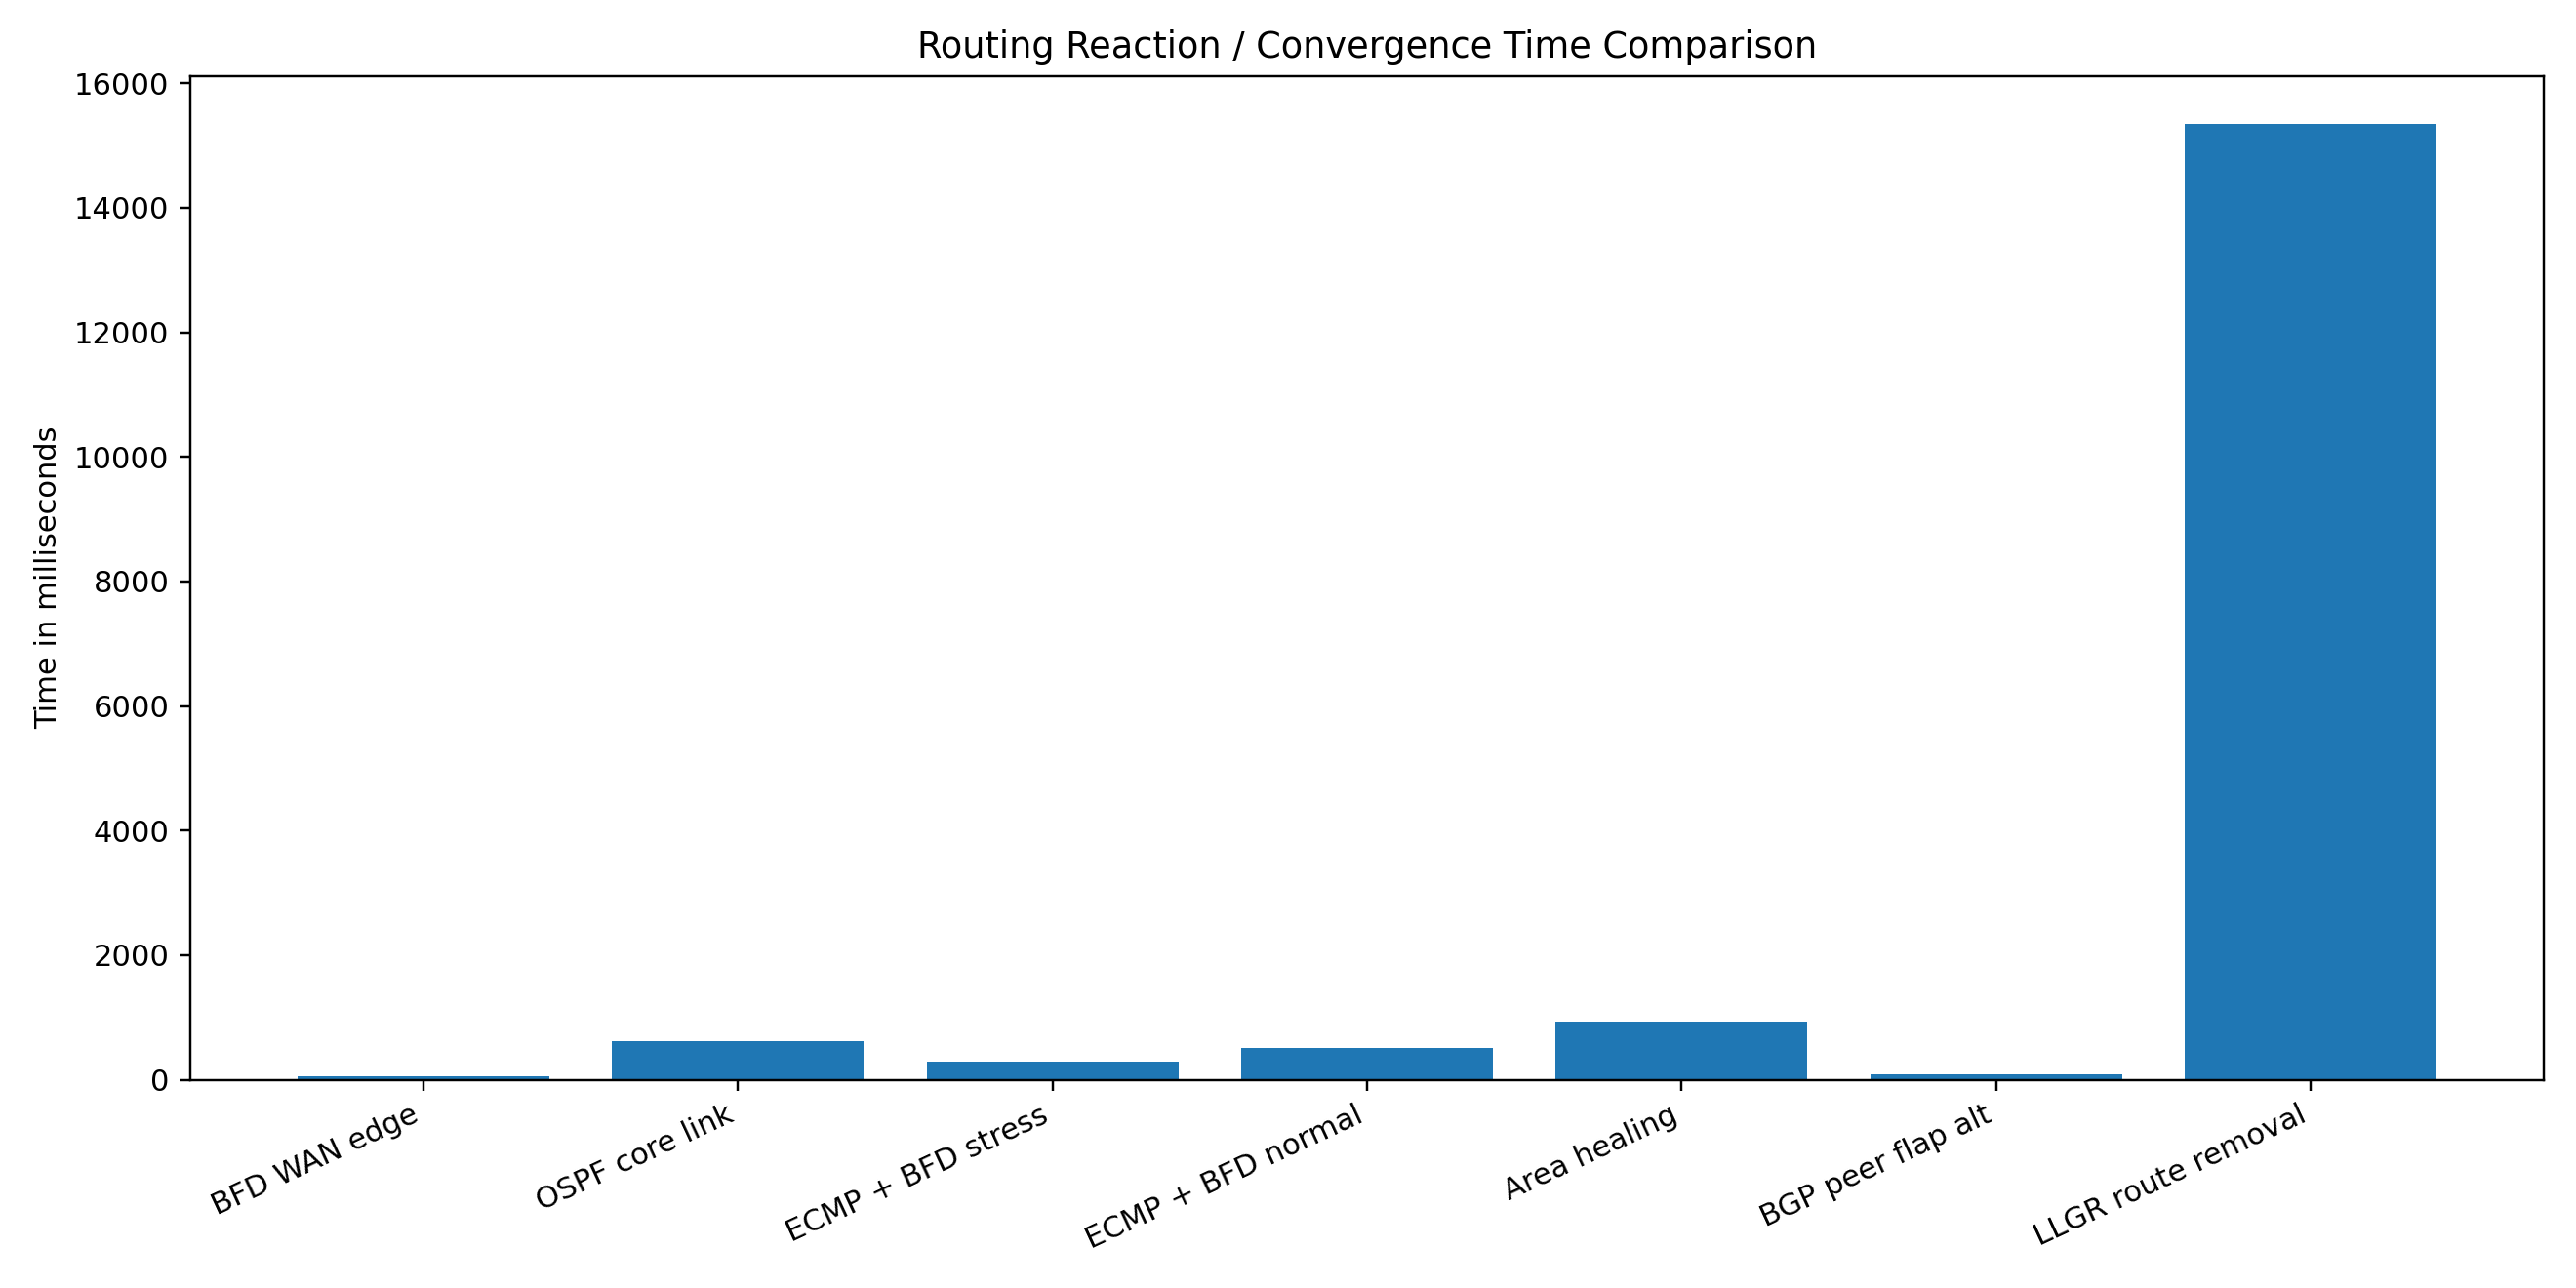
\includegraphics[width=0.95\textwidth]{figures/01_convergence_time_comparison.png}
\caption{Routing reaction and convergence time comparison}
\end{figure}

This graph compares the measured reaction or convergence time across different experiments. Lower values indicate faster failure detection or faster route recovery. The BFD WAN edge failure and BGP peer flap alternate-path switch showed very fast reaction times.

\subsection{Packet Loss Comparison}

\begin{figure}[H]
\centering
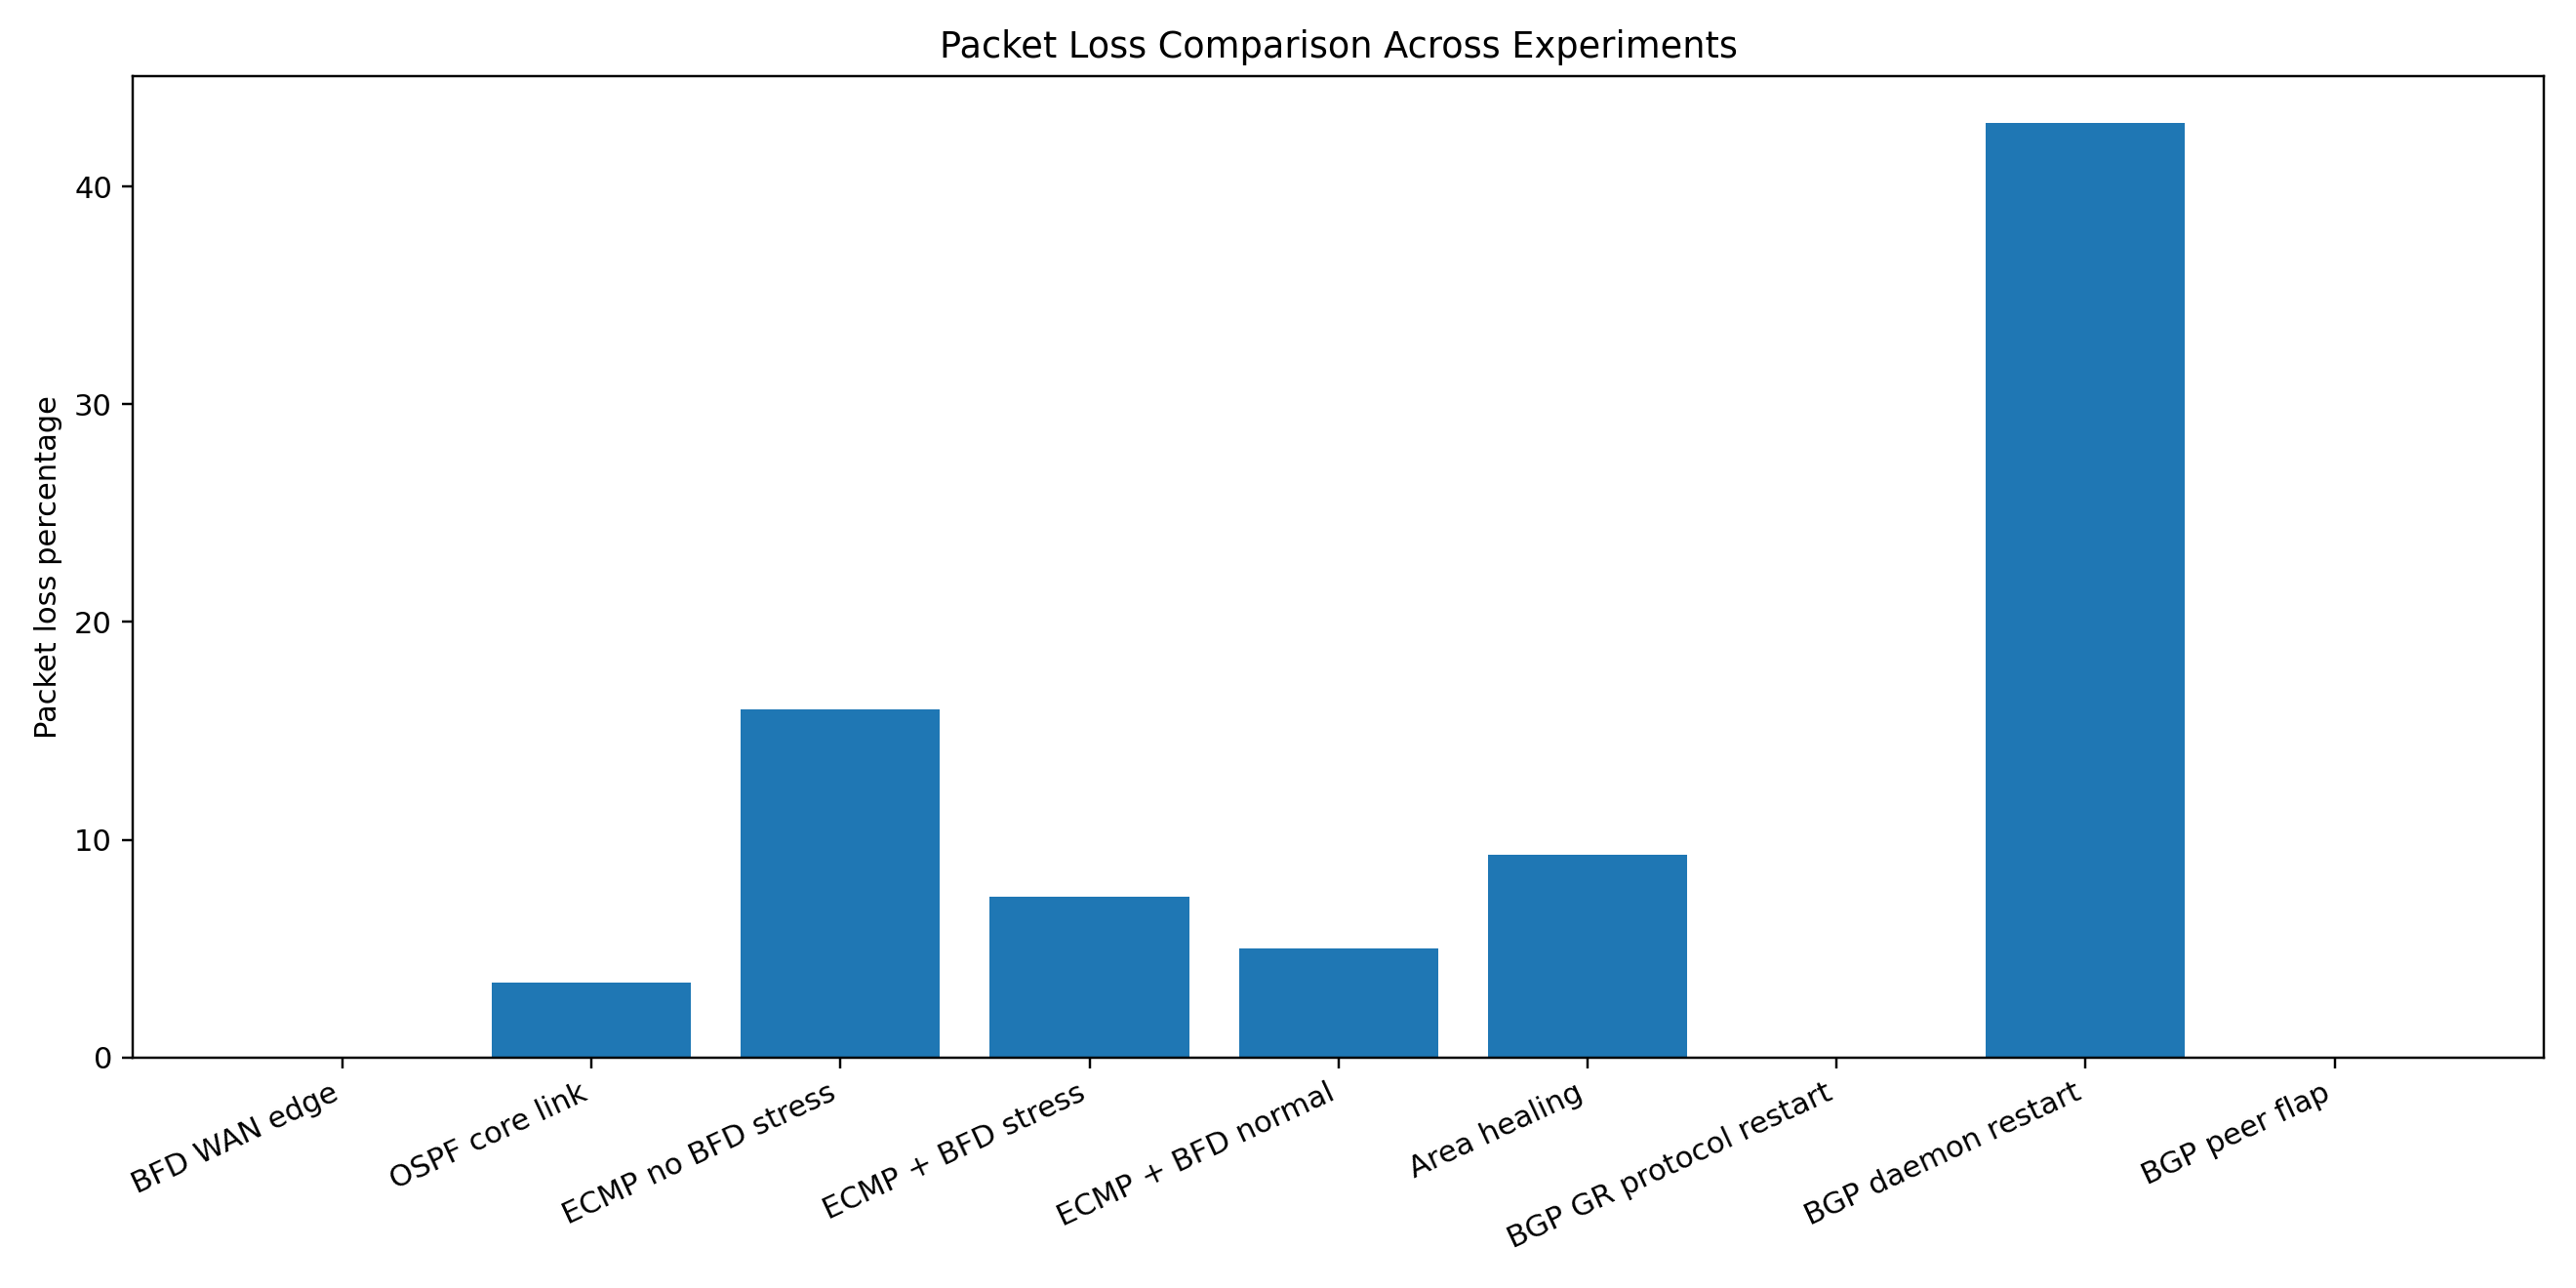
\includegraphics[width=0.95\textwidth]{figures/02_packet_loss_comparison.png}
\caption{Packet loss comparison across experiments}
\end{figure}

This graph compares the traffic impact during each experiment. The BFD WAN edge test, BGP GR protocol restart test, and BGP peer flap test preserved traffic with zero packet loss. The full BIRD daemon restart caused higher loss and is therefore reported as a limitation.

\subsection{Additional Deliverable Evidence}

\begin{figure}[H]
\centering
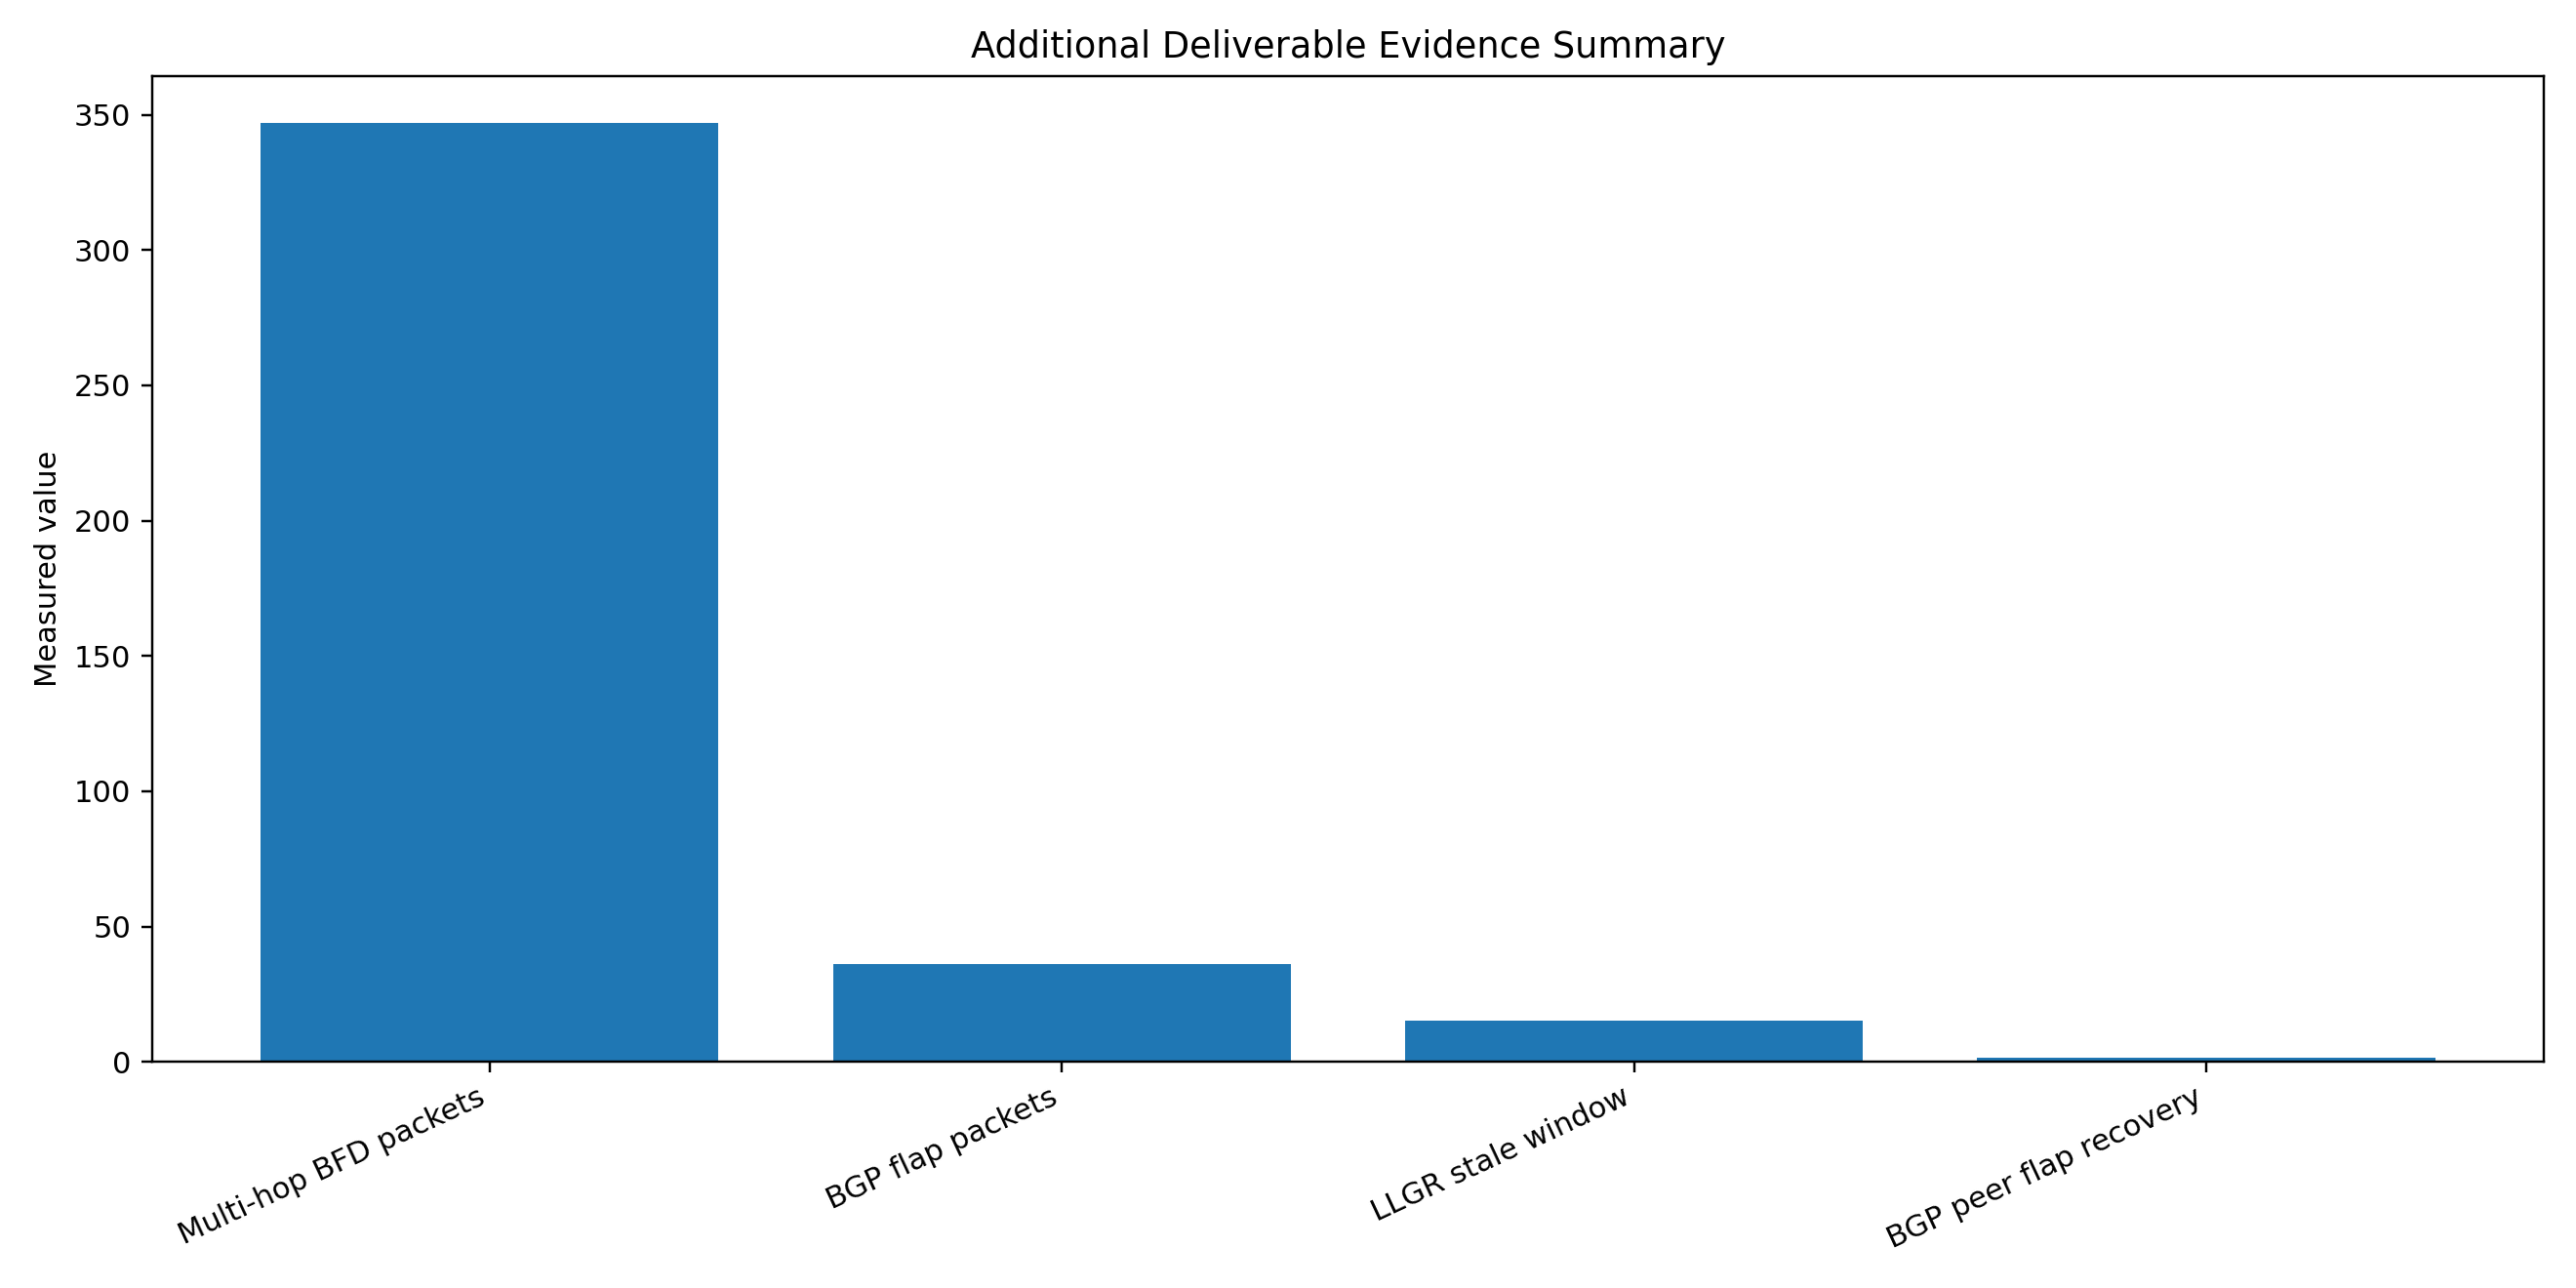
\includegraphics[width=0.95\textwidth]{figures/03_additional_deliverables_summary.png}
\caption{Additional deliverable evidence summary}
\end{figure}

This graph summarizes extra deliverables such as packet capture counts, LLGR stale-route timing, and BGP peer flap recovery. These results strengthen the project by adding packet-level validation and stale-route timer observation.
